% http://tex.stackexchange.com/questions/11866/compile-a-latex-document-into-a-png-image-thats-as-short-as-possible#11880
%http://tex.stackexchange.com/questions/152247/best-practice-to-include-standalone-precompiled-graphics
\documentclass[border=1pt]{standalone}
\usepackage{tikz}

\begin{document}

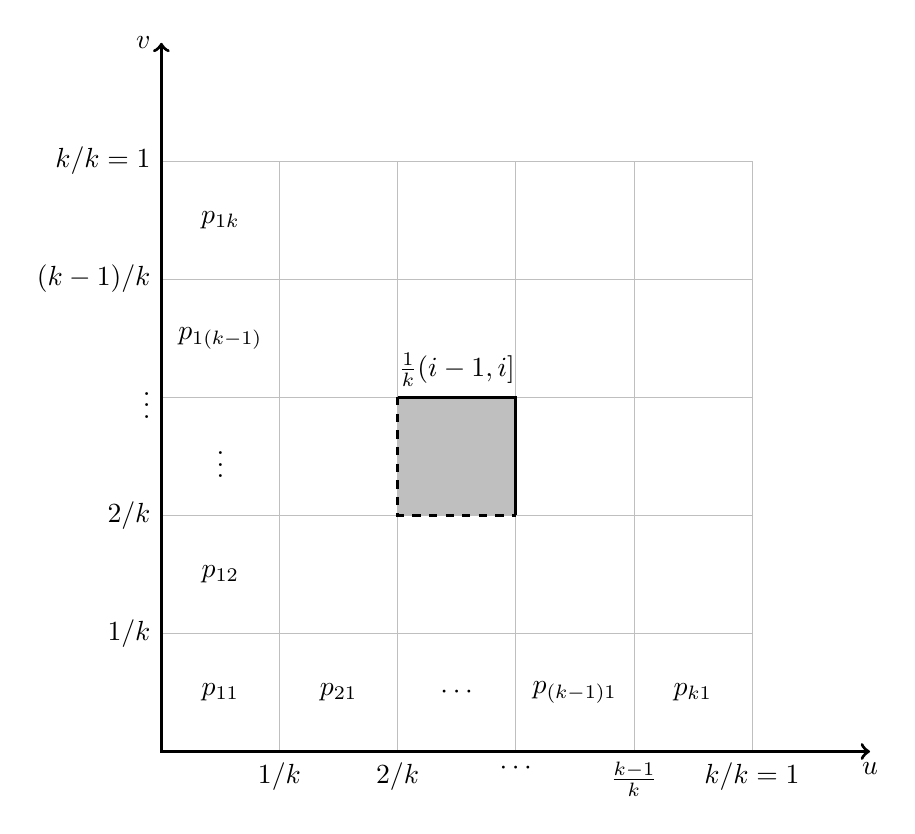
\begin{tikzpicture}[very thick, scale=1.5]
	\coordinate (A1) at (0,0);
	\coordinate (A2) at (5,5);
	\draw [help lines, lightgray] (A1) grid (A2);
	\draw[<->] (0,6) node[left] {$v$} -- (0,0) -- (6,0) node[below] {$u$};

	\node[left] at (0,1) {$1/k$};
	\node[left] at (0,2) {$2/k$};
	\node[left] at (0,3) {$\vdots$};
	\node[left] at (0,4) {$(k-1)/k$};
	\node[left] at (0,5) {$k/k = 1$};
	
	\node at (0.5,0.5) {$p_{11}$};
	\node at (0.5,1.5) {$p_{12}$};
	\node at (0.5,2.5) {$\vdots$};
	\node at (0.5,3.5) {$p_{1(k-1)}$};
	\node at (0.5,4.5) {$p_{1k}$};

	\node[below] at (1,0) {$1/k$};
	\node[below] at (2,0) {$2/k$};
	\node[below] at (3,0) {$\cdots$};
	\node[below] at (4,0) {$\frac{k-1}{k}$};
	\node[below] at (5,0) {$k/k = 1$};
	
	\node at (1.5,0.5) {$p_{21}$};
	\node at (2.5,0.5) {$\cdots$};
	\node at (3.5,0.5) {$p_{(k-1)1}$};
	\node at (4.5,0.5) {$p_{k1}$};

	\fill[lightgray] (2,2) rectangle (3,3);
	\draw[dashed] (2,3) -- (2,2)--(3,2);
	\draw         (2,3) -- (3,3)--(3,2);
\node[above] at (2.5, 3) {$\frac{1}{k}(i-1,i]$};

\end{tikzpicture}

\end{document}
